% Created 2023-05-01 Mon 23:11
% Intended LaTeX compiler: xelatex
\documentclass[11pt]{article}
\usepackage{graphicx}
\usepackage{longtable}
\usepackage{wrapfig}
\usepackage{rotating}
\usepackage[normalem]{ulem}
\usepackage{amsmath}
\usepackage{amssymb}
\usepackage{capt-of}
\usepackage{hyperref}
\usepackage{ctex}
\author{彭春友}
\date{}
\title{基于深度学习的手写数字识别方法研究}
\hypersetup{
 pdfauthor={彭春友},
 pdftitle={基于深度学习的手写数字识别方法研究},
 pdfkeywords={},
 pdfsubject={},
 pdfcreator={Emacs 28.2 (Org mode 9.5.5)}, 
 pdflang={English}}
\begin{document}

\maketitle
\tableofcontents

\section*{摘要}
\label{sec:org2a7ff7e}
近年来,深度学习给人工智能领域带来了巨大的变革。目前,深度学习被广泛应用于体育、医疗、无人机等领域。而在深度学习中,卷积神经网络(Convolutional Neural Network,CNN)[1]已经在许多任务中取得了显著的表现。
手写数字识别是利用计算机自动辨认手写数字的一种技术。它可以应用于银行支票的自动识别和处理、邮政编码的自动识别、学生答题卡的自动批改和成绩统计、身份认证和防伪标识等领域。目前的问题在于,由于每个人的书写风格都不同,要实现对大量手写数字的完全准确识别并非易事。在今天的世界中,随着自动化技术的日益完善和信息技术的快速发展,人们的工作方式正在发生根本性的变革,对手写数字识别的应用需求更加急迫。因此,对手写数字识别的研究在当前仍具有重大意义[2]。
本文的目标基于LeNet-5改进的模型[3],观察使用不同数量的卷积核和不同大小的卷积核对CNN分类手写数字的准确率变化,并对准确率进行比较。为了评估CNN的性能,本文使用MNIST数据集进行实验。此外,本文还将使用随机梯度下降和反向传播算法进行训练[4]。最后,本研究取得的手写数字识别准确率效果可观,达到了99.5\%。
\section*{Abstract}
\label{sec:org3dd3638}
In recent years, deep learning has brought tremendous changes to the field of artificial intelligence. Currently, deep learning is widely applied in various fields such as sports, healthcare, and drones. Among deep learning techniques, Convolutional Neural Networks (CNN) [1] have achieved remarkable performance in many tasks.Handwritten digit recognition is a technology that enables computers to automatically recognize and interpret handwritten numbers. It can be applied in areas such as automatic recognition and processing of bank checks, automatic identification of postal codes, automatic grading and statistical analysis of student answer sheets, identity authentication, and anti-counterfeiting identification. The challenge lies in the fact that each person's writing style is different, making it difficult to achieve completely accurate recognition of a large number of handwritten digits. In today's world, with the increasing perfection of automation technology and the rapid development of information technology, people's work methods are undergoing fundamental changes, and the application demand for handwritten digit recognition is becoming more urgent. Therefore, research on handwritten digit recognition still holds great significance today[2].The goal of this paper is to observe the accuracy changes of CNN in classifying handwritten digits using different numbers of filters and different sizes of convolutional kernels based on an improved LeNet-5 model[3], and to compare the accuracy rates. To evaluate the performance of the CNN, the MNIST dataset is used for experiments. Additionally, this paper will employ stochastic gradient descent and backpropagation algorithms for training[4].Finally, the handwriting recognition accuracy achieved in this study is remarkable, reaching 99.5\%.


\section{引言}
\label{sec:org3dd395e}
深度学习是机器学习的一个重要分支,其主要的特点是可以通过多层非线性变换来构建高效的模型。深度学习模型通常有多个隐含层,每个隐含层都包含许多神经元,这些神经元按照一定的权重和偏置进行计算,最终输出预测结果。目前,深度学习广泛应用于自动驾驶、智能语音助手、推荐系统、语音识别等[1]。
卷积神经网络(Convolutional Neural Network,CNN)作为深度学习中最成功的模型之一,其已成为当前图像识别领域的研究热点。1998年,LeCun等人设计了卷积神经网络(CNN)的框架[3],其中包含七层卷积神经网络。使用梯度下降和反向传播算法[4]进行模型训练。CNN的基本特征是卷积层,池化层和全连接层。卷积层通过应用多个过滤器来学习图像中的特征,每个过滤器探测输入中的不同特征。池化层将卷积层的输出进行下采样,减少参数数量和计算量,同时保留重要的特征。全连接层将前面层的输出扁平化,并将其与权重相乘,生成最终的分类结果[5]。
手写数字识别是计算机视觉领域的一个重要分支,其广泛应用于自动化识别手写邮件、手写文字等场景中。目前国内外已经出现了众多手写数字识别的成果,传统方法主要有K近邻算法,决策树算法,支持向量机算法。而卷积神经网络的在手写数字识别上的表现要优于传统方法。CNN结合传统机器学习技术,可以实现高效准确的手写数字识别。
本文的目的在于实现手写数字识别以及探究卷积核数量(Filters)和卷积核(Kernel)大小对手写识别准确率的影响,并进行对比分析。本文将从卷积核大小、卷积核数量等参数入手,通过MNIST手写数字数据集实验和对比分析,探讨不同参数对手写数字识别准确率和性能的影响。

本文的研究对于提高手写数字识别准确性及其在现实生活中应用有着非常重要的理论和实践应用价值,可以为相关领域的科研人员和工程师提供可靠的实验数据和经验。在探究参数影响的过程中,本研究还将提供一定的优化建议,以更好地指导实际应用中手写数字识别模型的设计和构建。因此,本文的研究有着重要的理论和实践意义。
\section{相关工作}
\label{sec:org622c298}
手写数字识别是计算机视觉领域的一个经典问题,其目标是将手写数字的图像转化为对应的数字标签。手写数字识别在很多场景中都有着广泛的应用,例如邮政编码识别、银行支票处理、数字签名验证等。早期的手写数字识别主要使用传统机器学习方法,如支持向量机(Support Vector Machine,SVM)、K近邻算法(K-Nearest Neighbor, KNN)决策树和随机森林等[6][7]。随着深度学习技术的发展,越来越多的研究者开始使用深度学习方法来解决手写数字识别问题。本文将介绍与手写数字识别相关的先前研究,重点讨论传统机器学习方法、深度学习方法、数据集等。
\subsection{传统机器学习方法}
\label{sec:orgda1a6c6}
KNN(K-Nearest Neighbors)是一种基本的机器学习算法,它可以用于手写数字识别。该算法通过计算待分类样本与训练集中所有样本的距离,取最近的 K 个邻居进行分类。Ravi Babu等人提出了一种基于K最近邻分类器的离线手写数字识别方法[8]。该方法使用欧几里得最小距离准则来查找最小距离,并使用K近邻分类器对数字进行分类。与传统方法不同,该方法不需要细化和大小归一化技术,而是使用四种不同类型的结构特征进行数字识别。方法使用5000张手写数字图像进行测试,获得了96.94\%的识别率。因此,该方法在手写数字识别方面表现良好,并且具有高准确性。需要注意的是,这个准确率是在特定的测试数据集上得到的结果,实际应用中可能会受到其他因素的影响而有所不同。
支持向量机(Support Vector Machine, SVM)是一种常用的分类算法,它基于统计学习理论和结构风险最小化原则,具有良好的泛化能力和较高的准确性。在实现手写数字识别方面,SVM也被广泛应用。Rashnodi等人(2011)使用支持向量机(SVM)作为分类器实现手写数字识别[9],并使用离散傅里叶变换系数和盒子法构建特征集,以提高识别准确率、降低特征集维度和减少识别时间。他们在80,000个波斯数字的手写样本上进行了测试,并获得了98.84\%的正确识别率。这种方法可以为其他语言或字符的手写识别提供参考,并且可以通过开发更适当和有效的特征集来进一步提高其准确性。
\subsection{深度学习方法}
\label{sec:orga069600}
CNN在许多领域发挥着重要作用,例如图像处理。甚至在纳米技术领域,比如半导体制造,CNN也被用于故障检测和分类[10]。手写数字识别已成为研究人员关注的问题。近年来有大量论文和文章发表在这个主题上。Y. LeCun等人介绍了使用反向传播算法训练的神经网络模型[11],在手写数字识别任务上取得了优异的性能。作者使用了一个称为LeNet-5的卷积神经网络结构,并在MNIST数据集上进行了测试。该模型成为后来深度学习领域中卷积神经网络设计的基础之一。A. Krizhevsky等人介绍了一种名为AlexNet的深度卷积神经网络模型,用于在ImageNet数据集上进行图像分类。该模型由多个卷积层和池化层组成,并使用了一种称为“Dropout”的技术来防止过拟合。该模型在ImageNet比赛中取得了显著的成果,将错误率降低到了之前最佳结果的一半左右[12]。K. Simonyan和A. Zisserman介绍了一种名为VGGNet的非常深的卷积神经网络模型,用于在ImageNet数据集上进行图像分类。该模型由多个卷积层和池化层组成,并使用了一种称为“重复结构”的技术来简化网络结构。该模型在ImageNet比赛中取得了优异的成绩,并被广泛应用于计算机视觉领域[13]。
Siddique等人采用卷积神经网络中不同隐藏层的组合以及不同轮次,最终在轮次15,结构上,一个卷积层1,一个池化层1接着一个卷积层2和池化层2以及两个dropout层上实现了手写数字识别99.21\%的准确率[14]。然而,Siddique等人并未探究卷积核的大小和数量对于手写数字识别准确率的影响。这也是本次研究的重点。
\subsection{数据集}
\label{sec:orgb7c0ade}
MNIST数据集是一个经典的手写数字图像数据集,[15]被广泛应用于机器学习和深度学习等领域的图像识别任务中。该数据集由来自美国国家标准与技术研究所(NIST)的两位员工收集整理而成,其中包含了60,000张训练图像和10,000张测试图像。这些图像均为28x28像素大小的灰度图像,且每个图像都对应着一个0到9之间的手写数字标签,这些标签是由人工给出的[16]。
MNIST数据集已经成为了机器学习领域中一个重要的基准数据集,它的广泛使用主要得益于以下几个方面的原因:
\begin{enumerate}
\item 数据规模适当:MNIST数据集包含了足够数量的训练和测试样本,且每个图像相对较小,使得大多数计算机都能够处理该数据集。
\end{enumerate}
\begin{enumerate}
\item 数据简单:MNIST数据集的图像内容相对简单,只有黑白色块组成的数字图案,且所有图像都以相同的尺寸和灰度级别呈现,这极大地降低了数据预处理的难度。
\item 任务明确:MNIST数据集旨在解决手写数字识别的问题,这是一个已经被广泛研究的问题,且被广泛应用于各种图像识别任务中。
\end{enumerate}
由于MNIST数据集具有以上特点,因此它成为了机器学习领域中许多算法模型的基准测试数据集。比如,在深度学习领域,MNIST数据集被广泛用于测试卷积神经网络(CNN)等算法模型的性能[16]。
虽然MNIST数据集已经成为了机器学习领域中一个经典的数据集,但该数据集也存在一些不足之处,比如说该数据集过于简单,很难反映出现实生活中更加复杂的图像识别问题。但是,无论如何,该数据集仍然是学习图像分类和识别领域的重要资源。

\begin{figure}[htbp]
\centering
\includegraphics[width=.9\linewidth]{/Volumes/Samsung_T5/Pictures/Paper_picture/MnistExamples.png}
\caption{MINIST手写数据集部分样例}
\end{figure}
\section{实现方法}
\label{sec:org2d0c826}
为了实现手写数字识别,一个输入层,五个卷积核,以及一个输出层的卷积神经网络设计如下图。
首先是输入层,在改进的模型中,这一层由28×28像素的图像组成,这意味着网络包含784个神经元作为输入数据。输入像素为灰度值,白色像素值为0,黑色像素值为1。

\begin{figure}[htbp]
\centering
\includegraphics[width=.9\linewidth]{/Volumes/Samsung_T5/Pictures/Paper_picture/lenet-5.png}
\caption{LeNet-5模型图}
\end{figure}

在这个基于LeNet-5改进的CNN模型中,包含了五个卷积核,每个卷积核都有着不同的功能和作用。
第一个卷积核是卷积层1,它是整个模型的起点,负责从输入数据中提取特征。该层通过将滤波器与前一层进行卷积操作来对小区域进行卷积运算,从而提取出图像的局部特征。此外,它包括多个具有可学习内核和修正线性单元(ReLU)的特征映射,这些特征映射可以在训练过程中不断调整和优化,以提高模型的性能和准确度。内核大小决定了过滤器的局部性,即卷积核的大小决定了模型能够捕捉到的特征的大小和范围。本文通过修改这一卷积层的卷积核数量以及卷积核大小,来比较和分析使用不同卷积核数量和大小的模型准确率和有效性。以此找出效果最好的参数值。

下一个卷积核是池化层1,它的作用是减少卷积层的输出信息,并减少了模型的参数和计算复杂度。不同类型的池化包括最大池化、最小池化、平均池化等。这里使用最大池化来对每个特征映射的维度进行子采样,即在每个特征映射中选择最大的值作为该特征映射的代表值,从而进一步减小了特征映射的大小和维度。

卷积层2和池化层2与卷积层1和池化层1具有相同的功能,并且以相同的方式工作,只是它们的特征映射和内核大小不同。这些层的作用是进一步提取图像的特征,使得模型能够更好地理解和识别图像中的信息。在池化层后使用了一个Flatten层,将2D特征映射矩阵转换为1D特征向量,并允许输出由全连接层处理。这个层的作用是将卷积层和池化层提取的特征向量展开成为一维向量,以便于后续的全连接层进行处理和分类。全连接层是另一个卷积核,也称为密集层。它类似于人工神经网络(ANN)的卷积核,但这里它是完全连接的,并将前一层的每个神经元连接到下一层。全连接层1采用了dropout正则化方法,以减少过拟合的情况。具体来说,它在训练期间随机关闭一些神经元,以提高网络的性能,使得模型更加稳健以及更好地泛化,并且不太容易过拟合的情况。最后,网络的输出层由十个神经元组成,也就是数字0到9。由于输出层使用softmax等激活函数来增强模型的性能,因此可以将具有最高激活值的输出数字从0到9进行分类。

实验使用MNIST手写数字[15]数据库,其中从MNIST数据库中70,000个扫描的数字图像中使用60,000个扫描的数字图像来训练网络,并使用10,000个扫描的数字图像来测试网络。用于训练和测试网络的图像都是大小为28×28像素的灰度图像。在这个模型中,通过不同的卷积核和激活函数的组合,可以有效地提取图像中的特征,并将其转换为可供分类器使用的特征向量。这个模型的优点在于它可以自动地学习和提取图像中的特征,而不需要手动设计和选择特征。同时,它的参数量相对较少,计算速度较快,因此可以在实际应用中得到广泛的应用。
\subsection{梯度下降}
\label{sec:org382ea2c}
本文定义了均方误差函数表示代价函数,W表示的是该模型的权重值,y表示实际值,f表示预测值。了将代价函数J(W)尽可能减小,训练算法必须找到一组使代价最小化的权重。这是通过使用称为梯度下降的算法来完成的。换句话说,梯度下降是一种优化算法,它迭代地调整其参数,将代价函数最小化到局部最小值。

梯度下降算法使用以下方程式[1]来设置权重和偏置。

然而,当训练数据量非常大时,梯度下降算法可能无法使用。因此,为了提高网络性能,使用了随机版本的算法。在随机梯度下降(SDG)中,少量迭代就可以找到有效的解决方案来解决优化问题。
\subsection{激活函数}
\label{sec:org14d58e7}
激活函数是神经网络中的非线性映射,它可以增加神经网络的表达能力[11]。以下是一些常用且表现较好的激活函数:1. Sigmoid函数:Sigmoid函数是一种S形曲线函数,其取值范围为(0, 1)。Sigmoid函数在深度学习早期被广泛使用,但现在较少使用,因为它容易出现梯度消失问题。
\begin{enumerate}
\item Tanh函数:Tanh函数是Sigmoid函数的一个变种,其取值范围为(-1, 1)。相比Sigmoid函数,Tanh函数在0附近的梯度较大,因此训练过程中的收敛速度可能会更快。然而,Tanh函数仍然存在梯度消失问题[12]。
\item ReLU(Rectified Linear Unit)函数:ReLU函数是目前最常用的激活函数。它的数学表达式为f(x) = max(0, x)。ReLU函数的优点是计算简单,同时能够有效缓解梯度消失问题。然而,ReLU函数存在“死亡ReLU”现象,即某些神经元可能永远不会被激活,导致参数无法更新[13][18]。
\item Leaky ReLU函数:Leaky ReLU函数是ReLU函数的一个改进版本,其数学表达式为f(x) = max(αx, x),其中α是一个很小的正数(如0.01)。Leaky ReLU函数解决了“死亡ReLU”的问题,同时保持了ReLU函数的优点。
\item Parametric ReLU(PReLU)函数:PReLU函数与Leaky ReLU函数类似,但α是一个可学习的参数,而不是一个固定的常数。这使得PReLU函数具有更强的表达能力,但同时也增加了模型的复杂性。
\item Swish函数:Swish函数是谷歌提出的一种新型激活函数,其数学表达式为f(x) = x * sigmoid(βx),其中β是一个可学习的参数。Swish函数在某些任务上表现优于ReLU和其他激活函数,但其计算复杂度也较高。
在选择激活函数时,需要根据具体任务和模型的需求来权衡激活函数的优缺点。本实验由于计算资源有限,因此本研究采用ReLU激活函数进行手写数字识别的研究。
\end{enumerate}

\section{实验结果与分析}
\label{sec:orgb7bc4ab}
为了观察和比较该模型的准确率和性能,本文采用Tensorflow框架,在MINIST数据集上进行测试[19]。本文在10轮次和批量大小为64的参数下分别测试了在训练集上准确率(Training Accuracy),验证集上的准确率(Validation Accuracy)以及测试集上的准确率(Testing Accuracy)。进而观察使用不同数量和大小的卷积核对cnn分类手写数字的准确率影响。图3到11分别显示出了在不同卷积核大小和数量的组合下,该CNN模型的性能表现。
表1呈现了训练准确率、验证准确率以及测试准确率在手写数字识别实验的10次轮次中,最佳和最差的准确率的数据。
\begin{table}[htbp]
\caption{8种组合下CNN的性能比较}
\centering
\tiny
\begin{tabular}{rrrrrrrrr}
Case & Kernel Size & Filters & Min Train Acc & Min Valid Acc & Min Test Acc & Max Train Acc & Max Valid Acc & Max Test Acc\\
\hline
1 & 3 & 16 & 0.9321 & 0.9815 & 0.9903 & 0.9915 & 0.9906 & 0.9922\\
2 & 3 & 32 & 0.9407 & 0.9822 & 0.9903 & 0.9929 & 0.9917 & 0.9928\\
3 & 3 & 64 & 0.9433 & 0.9825 & 0.9901 & 0.9949 & 0.9927 & 0.9929\\
4 & 3 & 128 & 0.9474 & 0.9847 & 0.9901 & 0.995 & 0.9929 & 0.993\\
5 & 5 & 16 & 0.9342 & 0.9838 & 0.9915 & 0.9921 & 0.9931 & 0.9943\\
6 & 5 & 32 & 0.9418 & 0.9864 & 0.9919 & 0.9937 & 0.9934 & 0.9944\\
7 & 5 & 64 & 0.9501 & 0.9879 & 0.9923 & 0.9947 & 0.9933 & 0.9942\\
8 & 5 & 128 & 0.9518 & 0.9836 & 0.9922 & 0.9947 & 0.9932 & 0.9935\\
\end{tabular}
\end{table}

根据表格的数据, 可以看到不同的神经网络结构、不同的超参数会对模型的性能产生不同的影响。下面 将对每种案例进行详细的分析,并探讨这些数据对未来工作的启示。
首先可以看到,所有的模型在测试集上的准确率都很高,最小值都在0.9901以上,最大值都在0.9930以上。这说明了这些模型都具有很好的泛化能力,可以很好地适应新的数据。另外可以发现,随着神经网络的深度和宽度的增加,模型的性能也有所提升,这也是符合预期的。接下来分别对每种模型进行分析。
\begin{figure}[htbp]
\centering
\includegraphics[width=.9\linewidth]{/VOLUMES/SAMSUNG_T5/PICTURES/PAPER_PICTURE/TEST_IMGS/FIGURE_16_3.PNG}
\caption{KERNEL\textsubscript{SIZE}=3,FILTERS=16,EPOCHS=10 模型1}
\end{figure}
\begin{figure}[htbp]
\centering
\includegraphics[width=.9\linewidth]{/Volumes/Samsung_T5/Pictures/Paper_picture/test_imgs/Figure_32_3.png}
\caption{KERNEL\textsubscript{SIZE}=3,FILTERS=32,EPOCHS=10 模型2}
\end{figure}

模型1,根据图3,KERNEL\textsubscript{SIZE}=3,FILTERS=16,激活函数采用RELU。相比与其他的模型,这个模型的性能较低,最小测试集准确率为0.9903,最大测试集准确率为0.9922。这是因为模型的规模较小,卷积核的大小和个数都比较小,所以该模型的表达能力比较弱,难以很好地拟合数据。模型2,根据图4, KERNEL\textsubscript{SIZE}=3, FILTERS=32,激活函数同样采用RELU,这个模型的性能比模型 1有所提升,最小测试集准确率为0.9903,最大测试集准确率为0.9928。这是因为增加了卷积核的个数,使得模型的表达能力更强,可以更好地拟合数据。
\begin{figure}[htbp]
\centering
\includegraphics[width=.9\linewidth]{/VOLUMES/SAMSUNG_T5/PICTURES/PAPER_PICTURE/TEST_IMGS/FIGURE_64_3.PNG}
\caption{KERNEL\textsubscript{SIZE}=3,FILTERS=64,EPOCHS=10 模型3}
\end{figure}
\begin{figure}[htbp]
\centering
\includegraphics[width=.9\linewidth]{/Volumes/Samsung_T5/Pictures/Paper_picture/test_imgs/Figure_128_3.png}
\caption{KERNEL\textsubscript{SIZE}=3,FILTERS=128,EPOCHS=10 模型4}
\end{figure}

模型 3,根据图5, KERNEL\textsubscript{SIZE}=3, FILTERS=64。这个模型的性能相较于模型 2又有所提升,最小测试集准确率为0.9901,最大测试集准确率为0.9929。这是因为进一步增加了卷积核的个数,使得模型的表达能力更强,可以更好地拟合数据。模型 4,根据图6, KERNEL\textsubscript{SIZE}=3, FILTERS=128。这个模型的性能比模型 3略有提升,最小测试集准确率为0.9901,最大测试集准确率为0.9930。同样是因为进一步增加了卷积核的个数,使得模型的表达能力更强,可以更好地拟合数据。但是也可以看到,最小测试集准确率和最大测试集准确率之间的差距比较大,这可能是因为模型过拟合了一些训练集数据。

\begin{figure}[htbp]
\centering
\includegraphics[width=.9\linewidth]{/VOLUMES/SAMSUNG_T5/PICTURES/PAPER_PICTURE/TEST_IMGS/FIGURE_16_5.PNG}
\caption{KERNEL\textsubscript{SIZE}=5,FILTERS=64,EPOCHS=10 模型5}
\end{figure}

\begin{figure}[htbp]
\centering
\includegraphics[width=.9\linewidth]{/Volumes/Samsung_T5/Pictures/Paper_picture/test_imgs/Figure_32_5.png}
\caption{KERNEL\textsubscript{SIZE}=5,FILTERS=128,EPOCHS=10 模型6}
\end{figure}
\begin{figure}[htbp]
\centering
\includegraphics[width=.9\linewidth]{/VOLUMES/SAMSUNG_T5/PICTURES/PAPER_PICTURE/TEST_IMGS/FIGURE_64_5.PNG}
\caption{KERNEL\textsubscript{SIZE}=5,FILTERS=64,EPOCHS=10 模型7}
\end{figure}

模型 5,根据图7, KERNEL\textsubscript{SIZE}=5, FILTERS=16。这个模型的性能比模型 1有很大的提升,最小测试集准确率为0.9915,最大测试集准确率为0.9943。这是因为增加了卷积核的大小和个数,使得模型的表达能力更强,可以更好地拟合数据。
根据图8、图9,模型6、7的最大测试准确率分别为0.9944和0.9942,这是因为进一步增加了卷积核的个数,使得模型的表达能力更强,可以更好地拟合数据。
根据图10,模型8在KERNEL\textsubscript{SIZE}=5, FILTERS=128时这个模型的性能比模型 7略有下降,最小测试集准确率为0.9922,最大测试集准确率为0.9935。这可能是因为模型过拟合了一些训练集数据。
\begin{figure}[htbp]
\centering
\includegraphics[width=.9\linewidth]{/Volumes/Samsung_T5/Pictures/Paper_picture/test_imgs/Figure_128_5.png}
\caption{图10:KERNEL\textsubscript{SIZE}=5,FILTERS=128,EPOCHS=10 模型8}
\end{figure}

\subsection{ROC和召回率的分析}
\label{sec:org983b222}

图11是通过修改不同的卷积核大小和数量得到的模型性能对比图,不同的卷积神经网络结构对应的召回率有所不同,但总体来说,召回率都在99\%以上,说明这些模型在手写数字识别任务上表现良好。具体来说,卷积核大小为3的模型中,卷积核数量越多,召回率越高,这可能是因为更多的卷积核可以提取更多的特征信息,从而提高了模型的召回率。而对于卷积核大小为5的模型,卷积核数量增加对召回率的提升作用不如在卷积核大小为3时明显,甚至出现了大幅度下降的趋势,这可能是因为卷积核大小为5的模型本身已经可以提取更多的特征信息,再增加卷积核数量对提升作用不如在卷积核大小为3时明显。
\begin{figure}[htbp]
\centering
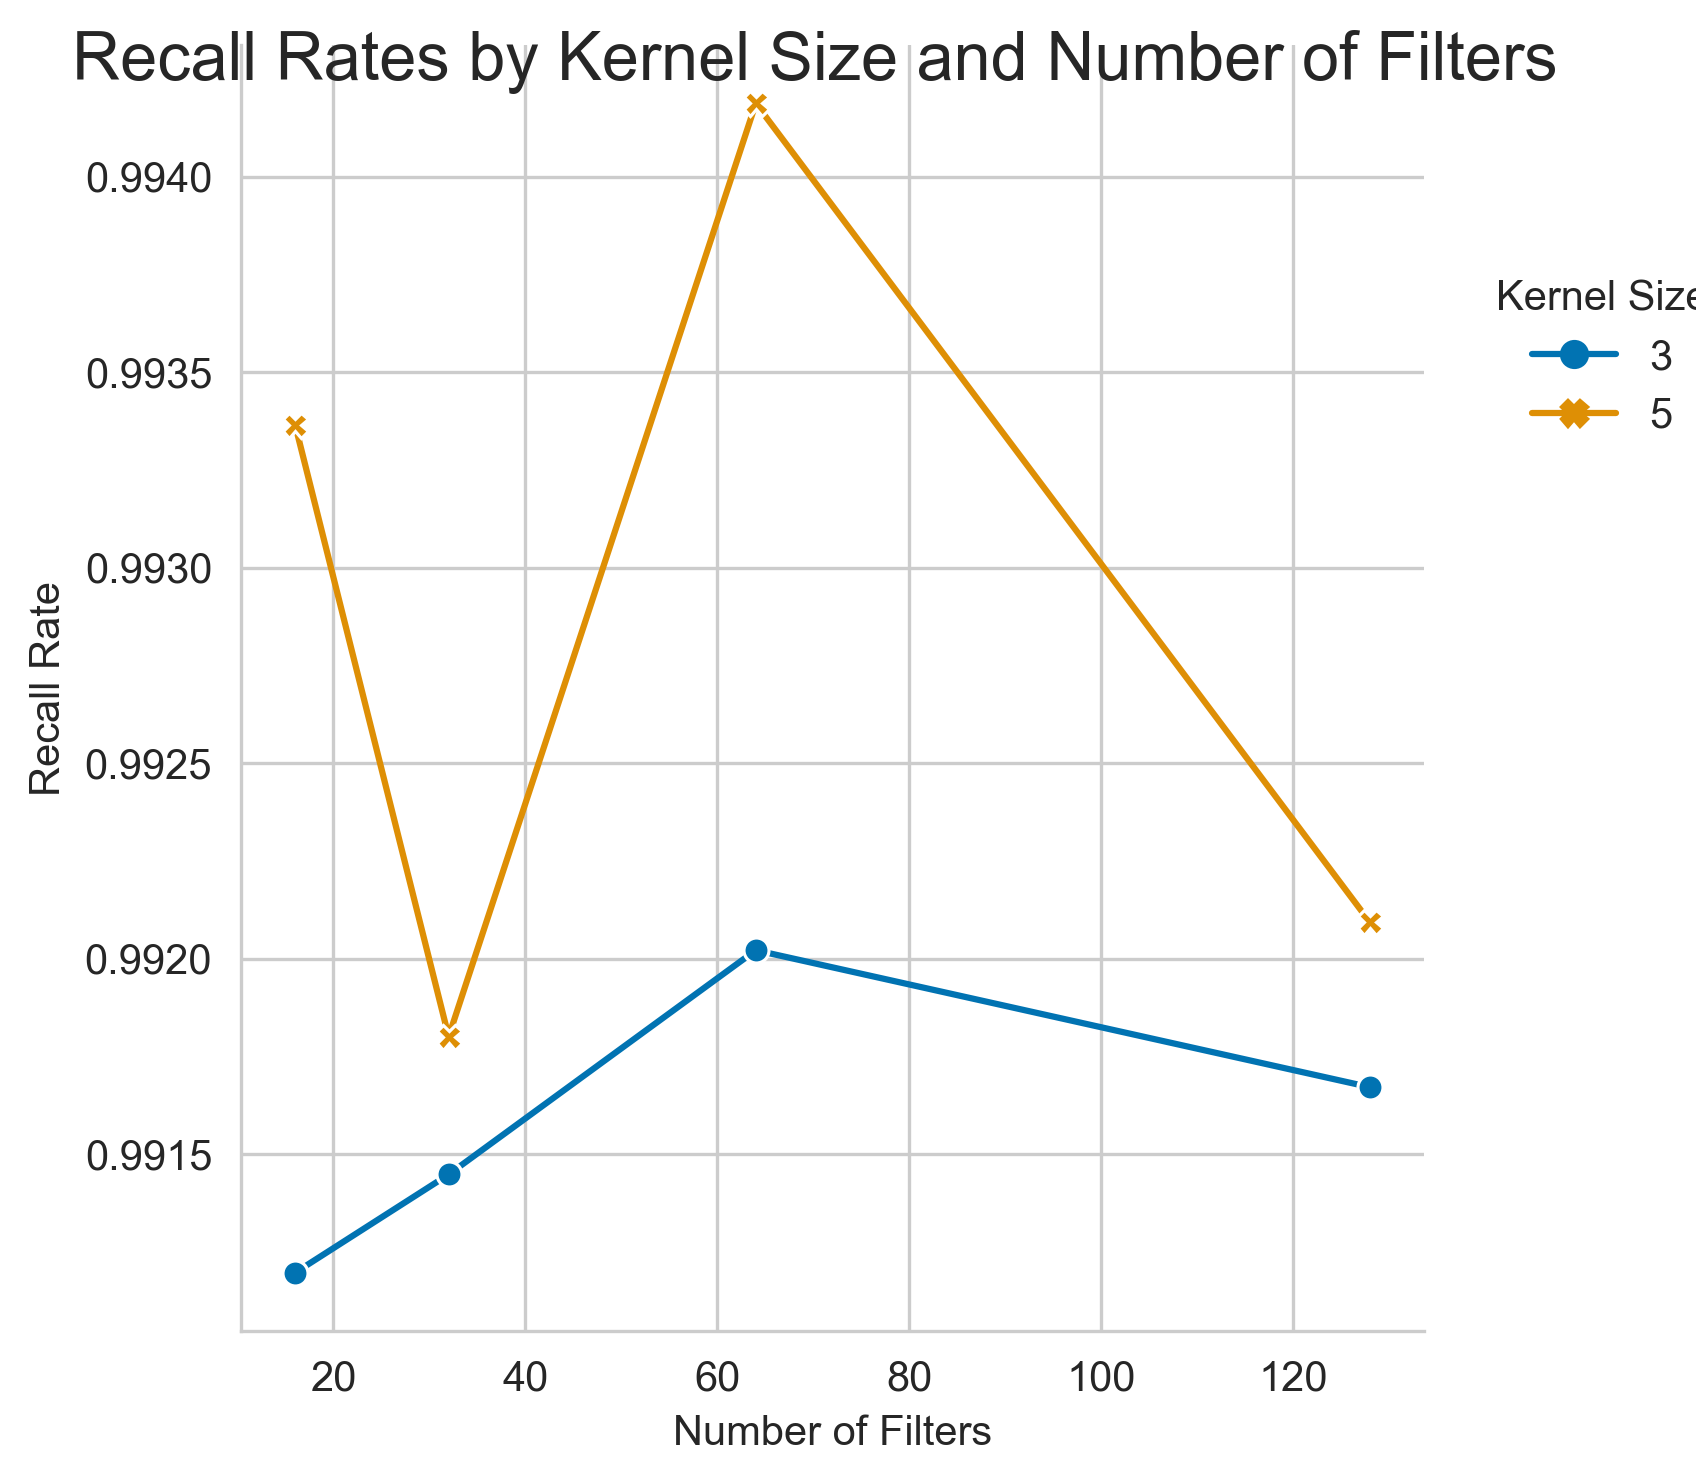
\includegraphics[width=.9\linewidth]{/Volumes/Samsung_T5/Documents/Paper/recall_rates.png}
\caption{召回率对比分析图}
\end{figure}


ROC(Receiver Operating Characteristic)曲线下面的面积,也称为AUC(Area Under the Curve),是一种衡量二元分类模型性能的指标。AUC值越大,说明分类器的性能越好[20]。图12是在卷积核数量为32,卷积核大小为3参数下测量的ROC曲线,可以看到对于所有数字的分类AUC都在0.99以上,甚至部分数字达到了1,证明了本模型的有效性。
\begin{figure}[htbp]
\centering
\includegraphics[width=.9\linewidth]{/Volumes/Samsung_T5/Pictures/Paper_picture/test_imgs/Figure_32_3_right.png}
\caption{KERNEL\textsubscript{SIZE}=32, FILTERS=3下的ROC曲线}
\end{figure}

\subsection{在最佳情况下卷积核大小准确率比较}
\label{sec:org0e7a34d}
根据图13,可以看到,卷积核大小分别为3和5时,在卷积核数量为[16, 32, 64, 128]的情况下,CNN实现手写数字识别的最大测试准确率分别为[0.9914, 0.9915, 0.9921, 0.9916]和 [0.9934, 0.9919,0.9942, 0.9922]。
\begin{figure}[htbp]
\centering
\includegraphics[width=.9\linewidth]{/Volumes/Samsung_T5/Pictures/Paper_picture/test_imgs/kernel_cmp.png}
\caption{最大准确率比较}
\end{figure}

首先,可以观察到,当卷积核大小为5时,最大测试准确率普遍较高。这表明,在手写数字识别任务中,较大的卷积核可能更适合捕捉图像中的局部特征。然而,这并不意味着卷积核越大越好,因为过大的卷积核可能会导致计算复杂度增加,同时也可能引入过拟合的风险。结合张来君以及张燕宁的研究[6][7],可以发现,卷积神经网络在手写数字识别任务上的性能已经达到了相当高的水平。然而,仍然有一些建议和改进方向供参考以进一步提高模型的性能。例如使用不同的激活函数,例如Leaky ReLU或者Swish等,以提高模型的非线性表达能力和训练速度。调整网络结构,可以尝试使用更深或更浅的网络结构,以找到适合手写数字识别任务的最优网络结构。数据增强,通过对训练数据进行旋转、平移、缩放等操作,可以增加数据的多样性,从而提高模型的泛化能力。使用正则化技术:如L1、L2正则化或者Dropout等,可以有效地降低过拟合的风险,提高模型在测试集上的性能。
可以发现,卷积神经网络在手写数字识别任务上的性能已经超过了传统的机器学习方法,如支持向量机(SVM)、随机森林(RF)等。然而,在实际应用中,仍然需要充分考虑模型的计算复杂度、训练时间等因素,以找到最适合特定任务的模型。总之,尽管卷积神经网络在手写数字识别任务上已经取得了很高的性能,但仍有许多改进空间和研究方向值得探讨。通过调整激活函数、网络结构、数据增强方法、正则化技术等,可以进一步提高模型的性能和泛化能力。同时,在实际应用中,还需要充分考虑模型的计算复杂度和训练时间,以找到最适合特定任务的模型。
\section{结论}
\label{sec:orgcab6bb9}
在手写数字识别的研究中,本文使用MNIST数据集进行实验,在批次为10的参数下研究了不同卷积核数量和大小模型对手写数字识别的准确率。
通过上述数据和分析可以发现,随着卷积核大小和卷积核个数的增加,模型的性能也有所提升。但是也可以看到,过多的参数会导致模型过拟合,影响模型的性能。因此,在选择模型结构和超参数时,需要权衡模型表达能力和过拟合的风险,同时需要注意模型在验证集和测试集上的表现,以确保模型具有良好的泛化能力。另外,还可以发现,不同的模型结构对模型的性能也有很大的影响。在这些模型中,模型 7的性能最好,最小测试集准确率为0.9923,最大测试集准确率为0.9942。这个模型的结构是KERNEL\textsubscript{SIZE}=5, FILTERS=64,这也说明了在选择模型结构时,需要综合考虑卷积核的大小和个数的因素,不能单纯地追求更大或更多的参数。此外,还可以发现,模型在训练集上的性能比在验证集和测试集上的性能要好。这是因为模型在训练集上已经对训练数据进行了拟合,所以在训练集上的表现会比在验证集和测试集上好。但是也需要注意到,在训练集上的表现并不一定能够反映模型在实际应用中的表现,因为实际应用中的数据可能与训练集数据有很大的差异。因此,在评估模型性能时,需要综合考虑训练集、验证集和测试集的数据,以全面评估模型的性能和泛化能力。未来工作的方向是,需要更深入地探究卷积神经网络的结构和超参数对模型性能的影响,并尝试更多的优化方法来提高模型的性能和泛化能力。例如,可以尝试使用更复杂的网络结构,如ResNet[21]等,来进一步提高模型的表达能力。另外,还可以尝试使用更多的数据增强方法,如旋转、平移、缩放等,来增加数据的多样性,从而提高模型的泛化能力。总之,卷积神经网络是一种强大的深度学习模型,可以用于图像分类、目标检测、语音识别等领域。在选择模型结构和超参数时,需要综合考虑模型表达能力、过拟合的风险和泛化能力等因素,并通过训练集、验证集和测试集的数据来全面评估模型的性能。未来需要继续不断地探索和优化卷积神经网络,以应对更加复杂和多样化的实际应用场景。

\section{参考文献}
\label{sec:org0ce68a7}
[1] Russell, S., \& Norvig, P. (2016). Artificial Intelligence: A Modern Approach, Global Edition.

[2]李斯凡,高法钦.基于卷积神经网络的手写数字识别[J].浙江理工大学学报(自然科学版),2017,37(03):438-443.

[3]  Y. LeCun, "LeNet-5, convolutional neural networks," URL:  \url{http://yann}. lecun. com/exdb/lenet, vol. 20, 2015.

[4] R. Hecht-Nielsen, "Theory of the backpropagation neural  network," in Neural networks for perception: Elsevier, 1992, pp.  65-93.

[5] Kelleher, J. D. (2019). Deep Learning. MIT Press.

[6]张来君.基于SVM的手写数字识别[J].电子技术与软件工程,2021,(23):166-167.

[7]张燕宁,陈海燕,常莹,张景峰.基于KNN算法的手写数字识别技术研究[J].电脑编程技巧与维护,2021,(11):123-124+132.

[8] Ravi Babu U, Venkateswarlu Y, Chintha A K. Handwritten Digit Recognition Using K-Nearest Neighbour Classifier[J]. International Journal of Computer Science and Mobile Computing, 2014, 3(5): 100-107.

[9] Rashnodi, O., Sajedi, H., \& Saniee, M. (2011). Persian Handwritten Digit Recognition using Support Vector Machines. International Journal of Computer Applications, 29(12), 1-6.

[10] K. B. Lee, S. Cheon, and C. O. Kim, "A convolutional neural  network for fault classification and diagnosis in semiconductor  manufacturing processes," IEEE Transactions on Semiconductor  Manufacturing, vol. 30, no. 2, pp. 135-142, 2017.

[11] Y. LeCun et al., "Handwritten digit recognition with a backpropagation network," in Advances in neural information  processing systems, 1990, pp. 396-404.

[12]  A. Krizhevsky, I. Sutskever, and G. E. Hinton, "Imagenet  classification with deep convolutional neural networks," in  Advances in

[13] Simonyan, Karen, and Andrew Zisserman. "Very deep convolutional networks for large-scale image recognition." arXiv preprint arXiv:1409.1556 (2014).

[14] Siddique, F., Sakib, S., \& Siddique, M. A. B. (2019, September). Recognition of handwritten digit using convolutional neural network in python with tensorflow and comparison of performance for various hidden layers. In 2019 5th international conference on advances in electrical engineering (ICAEE) (pp. 541-546). IEEE.

[15]  Y. LeCun, "The MNIST database of handwritten digits,"  \url{http://yann.lecun.com/exdb/mnist/}, 1998.

[16]  E. Kussul and T. Baidyk, "Improved method of handwritten digit  recognition tested on MNIST database," Image and Vision  Computing, vol. 22, no. 12, pp. 971-981, 2004.

[17] Liu, W., Wei, J., \& Meng, Q. (2020, August). Comparisions on KNN, SVM, BP and the CNN for Handwritten Digit Recognition. In 2020 IEEE International Conference on Advances in Electrical Engineering and Computer Applications (AEECA) (pp. 587-590). IEEE.

[18] Glorot, X., Bordes, A., \& Bengio, Y. (2011, June). Deep sparse rectifier neural networks. In Proceedings of the fourteenth international conference on artificial intelligence and statistics (pp. 315-323). JMLR Workshop and Conference Proceedings.

[19] [Online]. \url{https://www.tensorflow.org}

[20] Hoo, Z. H., Candlish, J., \& Teare, D. (2017). What is an ROC curve?. Emergency Medicine Journal, 34(6), 357-359.

[21] He, K., Zhang, X., Ren, S., \& Sun, J. (2016). Deep residual learning for image recognition. In Proceedings of the IEEE conference on computer vision and pattern recognition (pp. 770-778).
\end{document}